\section{Evaluation}
%\vspace{-1mm}
\subsection{Evaluation Methodology}
We implement both our architectures on Xilinx Alveo U280 FPGA. We use the ternary-quantized models from \cite{scalable} for inference performance evaluation. 
We first compare our performance and power consumption against a simplistic FPGA implementation of the ternary model~\cite{scalable} to show the benefits of our architectural designs. That basic design adopts a CPU-like architecture that only supports single-batch tasks while using off-chip memory to store the weights, which leads to a memory-bottlenecked implementation.

\begin{table}[h]
    \vspace{-3mm}
    \centering
    \caption{Attributes of the Evaluation Models}
    \label{tab:models} 
    \begin{tabular}{|r|r|r|r|}
        \hline
        Parameter& Dimension & Layer & Storage Size  \\
        \hline
        370M & 1K & 24 & 58MB \\
        \hline
        1.3B & 2K & 24 & 230MB \\
        \hline
        2.7B & 2.5K
        & 32 & 480MB \\
        \hline
        % 7B & 4k & 32 & 1.2GB \\
        % \hline
    \end{tabular}
    \vspace{-4mm}
\end{table}

To further highlight the performance of our design, we deploy the GPU baselines with the 370M model on NVIDIA Jetson Orin Nano, using TensorRT\cite{TensorRT} to maximize GPU performance. As the 1.3B and 2.7B models cannot fit into Jetson Orin Nano, we conduct experiments on NVIDIA's A100 GPU with TensorRT.  The models are quantized to the lowest supported precision for GPU deployment: INT8 for the Jetson Orin Nano and INT4 for the A100. While the model precisions on the GPUs differ from our ternary design, \cite{scalable} demonstrated that the models maintain high performance under ternary quantization. Although \textit{TerEffic} only accelerates the transformer blocks, our experiments show that the excluded layers (embedding layer, position encoding, and output layer) account for less than 0.1\% of the total GPU inference time, making the throughput comparison reasonable. 
\subsection{FPGA Resource Utilization}
\vspace{-0.5mm}
We perform synthesis on Vivado v2022.1 and achieve \textbf{250MHz} frequency. The resource utilization of the On-Chip Architecture is presented in Table \ref{tab:table2}, while the HBM-Assisted version is the same except for the inclusion of HBM.
\begin{table}[h]
    \centering
    \vspace{-3mm}
    \caption{\textit{TerEffic} FPGA Resource Utilization}
    \label{tab:table2} 
    \vspace{-1mm}
    \resizebox{\linewidth}{!}{
    \begin{tabular}{|r|r|r|r|r|r|r|}
        \hline
        LUT & Reg & Carry8 & Mux & DSP & BRAM & URAM \\
        \hline
        862K & 700K & 82K & 542K & 1,551 & 385.5 & 865 \\
        \hline
        66.12\% & 26.88\% & 50.13\% & 83.03\% & 17.19\% & 19.12\% & 90.10\% \\
        \hline
    \end{tabular}
    }
    \vspace{-3mm}
\end{table}

As our FPGA design adopts customized TMUs made up of LUTs and Muxes, their utilizations are significantly higher than that of costly DSPs. Moreover, as discussed in Section \ref{sec:Compute-Memory Alignment}, we choose URAM to store weights instead of BRAM, which accounts for the high URAM utilization and low BRAM utilization.


\subsection{On-Chip Architecture Evaluation}
%throughput
The single-batch latency of the on-chip architecture for the 370M model is $820\times 24 \text{ layers} = 19680 \ cycles$, leading to a single-batch throughput of \textbf{$\approx$12,700 tokens/sec}. With \textbf{pipeline parallelism}, the maximum batch size for the 2-card system is 20 and the multi-batch throughput is thereby \textbf{$\approx$130,200 tokens/sec}. As only activations are transmitted between the two cards, the inter-card communication overhead is negligible and not included.

We estimate power for one card using Vivado as $P_0=23.5W$. A detailed power breakdown is shown in Fig. \ref{fig:powerbreakdown}, where  CLB contains LUT, Regs, muxes and other logic, and Sig\&Clk denotes signals and clock. The majority of power consumption originates from the URAM due to frequent weight transfer, underscoring the importance of our hybrid memory architecture. Moreover, CLB consumes little power (4\%) despite handling most of the computational workload, emphasizing the high efficiency of the TMUs.
\begin{figure}
    \centering
\resizebox{\linewidth}{!}{
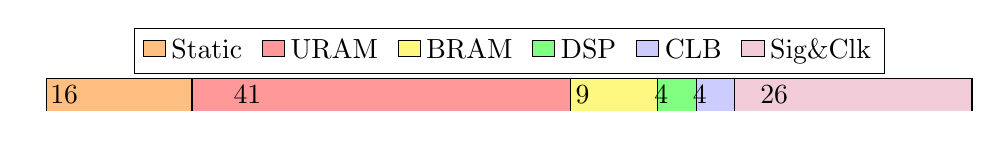
\begin{tikzpicture}[]
    \begin{axis}[
    xbar stacked,
    width=1.1\linewidth,
    xmajorgrids = true,
    xmin=0,xmax=100,
    ytick style={draw=none},
    ytick = data, yticklabels = {},
    bar width=6mm, y=10mm,
    nodes near coords={}, % <-- prints % sign after y coordinate value
    % xticklabel={\pgfmathprintnumber{\tick}\%},% <-- prints % sign after x tick value
    nodes near coords align={}, % <-- horizontal alignment centered of nodes 
    enlarge y limits=0.5, % <-- Adds vertical space so to not crop the bars
    % legend style={font={\fontsize{12 pt}{12 pt}\selectfont}},
    legend style={/tikz/every even column/.append style={column sep=0.18cm}},
    % legend image post style={xscale=1.5, yscale=1},
    legend columns =6,
    legend style={at={(0.5,1.15)},anchor=south},
    % legend image code/.code={
    % \draw [/tikz/.cd,bar width=3pt,yshift=-0.2em,bar shift=0pt]
    %         plot coordinates {(0cm,0.8em)};
    %     },
    xtick=\empty
    ]
        \addplot [fill=orange!50,nodes near coords align={xshift=-7mm},nodes near coords={16}] coordinates{(15.7,1)};
        \addplot [fill=red!40,nodes near coords align={xshift=-17mm},nodes near coords={41}] coordinates{(40.9,1)};
        \addplot [fill=yellow!50,nodes near coords align={xshift=-4mm},nodes near coords={9}] coordinates{(9.4,1)};
        \addplot [fill=green!50,nodes near coords align={xshift=-2mm},nodes near coords={4}] coordinates{(4.2,1)};
        \addplot [fill=blue!20,nodes near coords align={xshift=-2mm},nodes near coords={4}] coordinates{(4.1,1)};
        \addplot [fill=purple!20,nodes near coords align={xshift=-10mm},nodes near coords={26}] coordinates{(25.6,1)};
        \legend{Static,URAM,BRAM, DSP,CLB, Sig\&Clk}
    \end{axis}
\end{tikzpicture}
}
\caption{FPGA Power Breakdown (\%) for the on-chip design }
    \label{fig:powerbreakdown}
    \vspace{-7mm}
\end{figure}

When the 2-card system is executing a single-batch task, only one card is active, while the other remains idle and only consumes 3.7W static power ($P_{static}$). Therefore, the overall power estimation is $P_0+P_{static}=\mathbf{27.2W}$. In contrast, when running multi-batch tasks, the inputs are executed in a pipeline manner and all cards contribute to full power consumption, leading to $P=2\times P_0=\mathbf{47.0W}$. 

\begin{table}[h]
    \vspace{-1mm}
    \centering
    \caption{Comparison of \textit{TerEffic} (On-Chip) with GPU and a simplistic FPGA design\cite{scalable} for a 370M model.}
    \label{tab:onchip_comparison} 
    \resizebox{\linewidth}{!}{
    \begin{tabular}{|r|r|r|r|r|r|r|r|}
        \hline
        Hardware& Batch &TP & TP& Power& Eff &Eff \\
        & Size &(tk/s)& Impv& (W) & (tk/s/W) & Impv\\
        \hline
        FPGA\cite{scalable}  &  1&  62& 0.7$\times$ & 13.7 &5 & 0.2$\times$ \\
        \hline
        Jetson  &  1& 85& 1$\times$ & 3.5 &24 & 1$\times$ \\
        \hline
        \textit{TerEffic} &  1&  12,700& 149$\times$&  27.2&467& 19$\times$ \\
        \hline
        \hline
        Jetson  & 20&  1,096&1$\times$&  4.6 & 240& 1$\times$ \\
        \hline
        \textit{TerEffic}  &  20&  130,200&119$\times$&
        47.0&2,770& 12$\times$ \\
        \hline
    \end{tabular}
    }
    \vspace{-3mm}
\end{table} 
We compare our on-chip results on the 370M model with the FPGA results from \cite{scalable} and the experimental results on Jetson Orin Nano, with the GPU batch size set to 1 and 20 to match our design (see Section \ref{sec:On-Chip Architecture}). The comparison is presented in TABLE \ref{tab:onchip_comparison}, where TP denotes throughput (tokens/sec), Eff denotes power efficiency (tokens/sec/watt) and TP/Eff Impv denotes the throughput/efficiency improvement over Jetson Orin Nano. While the basic ternary FPGA design~\cite{scalable} is not competitive, \textit{TerEffic} significantly outperforms the edge GPU in terms of both throughput and power efficiency, achieving $\mathbf{149\times}$ throughput and $\mathbf{19\times}$ power efficiency in single-batch tasks. When processing multi-batch tasks, our design exceeds the GPU's throughput and power efficiency by $\mathbf{119\times}$ and $\mathbf{12\times}$, respectively. These impressive improvements highlight the exceptional efficiency of our on-chip architecture, fully utilizing the massive on-chip bandwidth compared to the GPU's off-chip DRAM. Moreover, while GPUs lack low-precision support, our customized TMUs unlock substantial computational capabilities through efficient ternary operations.
 



\subsection{HBM-Assisted Architecture Evaluation}
The HBM-assisted architecture is used to accelerate larger models with a single card. As discussed in Section \ref{sec:HBM-Assisted Architecture}, the single-batch latency is 2,400 cycles/layer for the 370M model, and the throughput is thereby 4,340 tokens/s. By leveraging the \textbf{full-resource parallelism}, a maximum batch size of 15 is supported regardless of the model size, and the multi-batch throughput is $\approx$ 60,000 tokens/s. As the HBM-assisted latency is constrained by the HBM bandwidth, the throughput will decrease to $\frac{1}{n}$ when the model size increases by $n\times$. 

The HBM power is estimated as $P_{HBM}=9.2W$. Therefore, the overall power  is $P=P_0+P_{HBM}=\mathbf{32.7W}$. Since the resource remains unchanged for varying model sizes, the power consumption can be considered constant. We compare our results with the basic FPGA results\cite{scalable} on the 1.3B model, and conduct A100 experiments on the 1.3B and 2.7B models, with the batch size set to 1 and 15 to match our design (see Section \ref{sec:HBM-Assisted Architecture}). The results are presented in TABLE \ref{tab:HBM_comparison}. 

\begin{table}[h]
    \vspace{-2mm}
    \centering
    \caption{Comparison of \textit{TerEffic} (HBM-assisted) architecture with GPU and a basic FPGA design\cite{scalable} for larger models}
    \label{tab:HBM_comparison} 
    \resizebox{\linewidth}{!}{
    \begin{tabular}{|r|r|r|r|r|r|r|r|}
        \hline
        Model, &Hardware &TP & TP& Power&Eff &Eff \\
        Batch Size& &(tk/s)& Impv& (W)&(tk/s/W) & Impv\\
        \hline
        1.3B,1&FPGA\cite{scalable}  &  24& 0.05$\times$& 13.9 &2 & 0.5$\times$ \\
        \hline
        1.3B,1&A100  &  499& 1$\times$ & 119.6 &4 & 1$\times$ \\
        \hline
        1.3B,1&\textit{TerEffic}  &  1,085& 2$\times$&  32.7&33& $8\times$ \\
        \hline
        \hline
        1.3B,15&A100  &  6,757& 1$\times$ & 131.6 &51 & 1$\times$ \\
        \hline
        1.3B,15&\textit{TerEffic}  &  15,000& 2$\times$&  32.7&459& $9\times$ \\
        \hline
        \hline
        2.7B,1&A100  & 250&1$\times$& 124.0 & 2& 1$\times$ \\
        \hline
        2.7B,1&\textit{TerEffic} &521&2$\times$&
        32.7&16& 8$\times$ \\
        \hline
        \hline
        2.7B,15&A100  & 3,433&1$\times$& 138.3 & 25& 1$\times$ \\
        \hline
        2.7B,15&\textit{TerEffic} &7,200&2$\times$&
        32.7&220& 9$\times$ \\
        \hline
    \end{tabular}
    }
\end{table} 

Although the HBM-assisted architecture lacks the benefits of on-chip inference, our design still achieves significantly higher efficiency than GPUs by leveraging the advantages of ternary LLMs. For multi-batch tasks, where GPUs typically excel, our design is enhanced by the \textbf{full-resource parallelism} and continues to deliver superior performance. While the A100 can handle a massive batch size, a batch size of 15 is sufficient for typical edge tasks, where throughput with smaller batch sizes becomes more critical.

\subsection{Further Estimations on 7B Model}
 Based on the previous results, we estimate the performance on a 7B model, which is a commonly used LLM size. Our HBM-assisted design is estimated to deliver a single-batch throughput of $\approx$ 200 tokens/sec with a power consumption of 33W, comparable to the typical power usage of a personal laptop. 
 In comparison, FlightLLM\cite{flightllm}, one of the state-of-the-art FPGA LLM accelerators, achieved a throughput of 55 tokens/sec for a 7B model on the same U280 FPGA by leveraging sparsity. Apple’s newly launched M4 Max, which is specifically optimized for local AI deployment, is estimated to achieve 100 tokens/sec in inference for an 8B model\cite{AppleM4}. Given that our FPGA is based on the 16nm process while the Apple M4 Max uses the 3nm process, our HBM-assisted design can achieve 10$\times$ better power efficiency projected on the same technology node. With larger on-chip memory and further development of model compression techniques, our on-chip architecture has the potential to deliver even greater performance. 
 Other high-performance LLM accelerators, such as Cerebras\cite{cerebras_1} and Groq\cite{groq}, have also benefited from on-chip inference and achieved remarkable throughput of several thousand tokens per second\cite{cerebras_3}. However, these chips utilize massive on-chip SRAM (e.g., 44GB for Cerebras WSE-3 engine\cite{cerebras-2}) and consume substantial energy as high as several kilowatts, which confines their use to data centers rather than edge environments. 



\section{Conclusion}

We have introduced \textit{TerEffic}, an FPGA-based accelerator designed to enable efficient on-chip LLM inference by leveraging the benefits of ternary quantization. Our key innovations --- 1.6-bit weight compression, specialized TMUs, and compute-memory alignment --- enable unprecedented efficiency for edge deployment while preserving accuracy. The fully on-chip architecture excels at processing smaller models, while the HBM-assisted variant extends support to larger models with strong performance. Our work establishes a foundation for future research in hardware-efficient LLM deployment, particularly in resource-constrained environments where power efficiency is paramount.
\vspace{-0.5mm}
